\chapter{Web Testing with Selenium 2}

\section{Examples}
The aim here is to write a program that tests another program that the tester has no idea of its code. Selenium's API can be thought of as instructions for a browser that performs the tests. First, the tester must make the test plan. Then, (s)he prepares the test cases. Finally, the test cases are converted into a Java program that is written with Selenium API to instruct the browser to perform the tests.

\subsection{Additional Exercise with Selenium}
In this exercise, you are expected to test the number of CMPE courses available on Moodle using Selenium. You should open the Moodle web page, click on “Moodle Courses”, search for “cmpe” and get the number next to the search results text. The location of the number of courses after a search is displayed in \reffig{num-search-results}. To reach that number:

\begin{figure}
    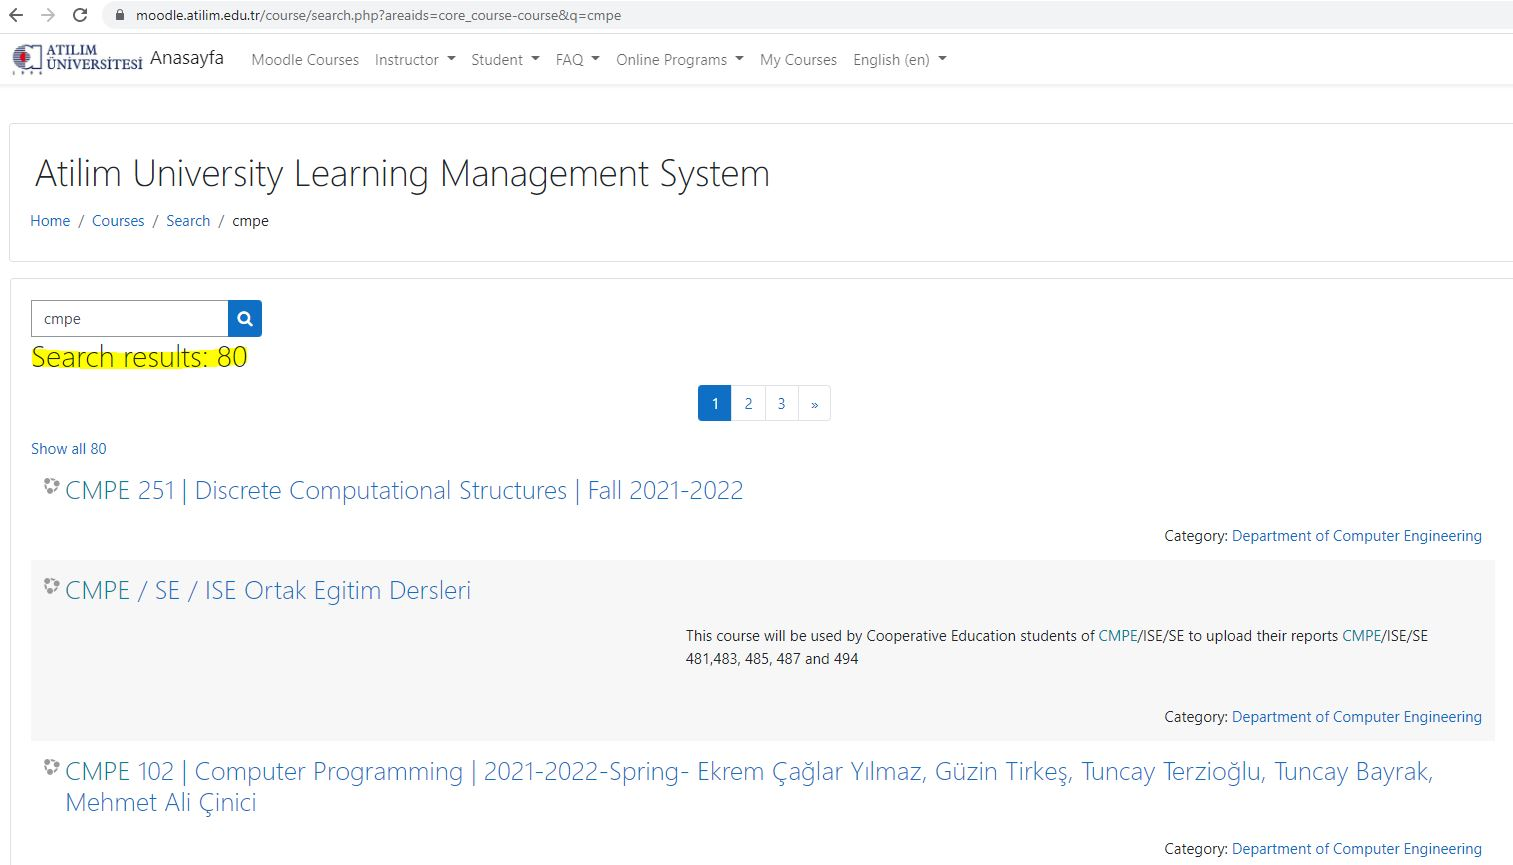
\includegraphics{images/selenium1-detailed-install-3.jpg}
    \caption{Number of search results on the Moodle web page.}
    \labfig{num-search-results}
\end{figure}

\begin{enumerate}
    \item You should get the xpath of the web element that the number is in.
    \item Using that xpath, you should get the text of that web element.
    \item Since the text will be something like “Search results: xxx” and we only need the number there, you should extract the digit part of that text.
    \item The data type of extracted digits will be string by default. So finally, to be able to store the number in an integer variable and compare with the expected result, you should convert it to integer.
\end{enumerate}

After comleting all the steps listed above, create a test class in the src/test/java folder.  Write the code below inside the class and run as Maven test.

\todo{Kod gelecek.}

\subsection{Testing Atılım University Moodle Page}
Like other universities, Atılım University has a Learning Management System (LMS) called Moodle. Moodle is an open-source LMS system that is supported by more than 600 contributors worldwide\sidenote{\url{https://github.com/moodle/moodle}}. That is all by itself guarantees that Moodle is well tested and documented. For demonstration purposes, we are going to test some of the functionality of Moodle with black-box testing strategies.

Let's start with creating a Maven project as described in Chapter \ref{lab:introduction}. This time remember to include Selenium as a dependency as described in the previous section. We will test two functionality as a warm-up practice. The first one is about testing the login link to see if the login page is successfully loaded. The second one is about checking if the SE344 course page can be searched and found through the course searching mechanism. Write the following code snippet and we will discuss the important statements later.

\lstinputlisting[language=java,caption={Testing Moodle with a few warm-up tests.},label=lst:test-moodle]{code-snippets/TestMoodle.java}

In the Listing \ref{lst:test-moodle}, we have two tests, one initialization method, and one tear-down method. The initialization method \lstinline!static void initAll()! opens and prepares a web driver which is in type \lstinline!ChromeDriver()!. This means that the driver will open a Google Chrome instance. It does that only once and assumes that WebDriver executable can be found in \lstinline[language={}]!PATH!. After that, the tests are going to run.

The \lstinline!testLogin()! test method starts with opening up the Moodle page (29). Then, it finds an anchor (link) which has a \emph{Log in} text in it via the anchor's XPath (30). XPath is a query language for querying markup languages such as HTML, XML, etc. More information about XPath can be found in Appendix \ref{ch:appendix-xpath}. After finding the link, click on it (31) and wait for a button with an id of \emph{loginbtn} to appear (32). When it appears, check if its text is \emph{Log in} (34).

The \lstinline!testSE344Course()! test method reopens the main page of Moodle (40). In line (41), we create a \lstinline!WebDriverWait! object \lstinline!wait! which we will use for explicit waits to a maximum of 10 seconds. After that, we find the \emph{Moodle Courses} link by its XPath (43) and click it (44). In the upcoming page, we choose the input field again by its XPath (46) that allows us to search \emph{SE 344} (47) and press \keys{\return} (48). After getting the desired page, we look for the text \emph{System Software Validation and Testing} on the page (50). If we find it, then the test passes.

Finally, the \lstinline!static void tearDownAll()! method run after all the tests are finished. The method checks if the driver is initialized (56) and if so, it closes it with its \lstinline!close()! method (57). This method also closes the opened browser window.
